\chapter{Sword Mage}

{\color{red}  \textbf{NOTE:} any text in red is related to design decisions. It might be useful for discussion.}    

\begin{table*}[ht!]
\begin{small}
\rowcolors{2}{}{commentgreen}
\begin{center}
\begin{tabular}{ccccllllll}
\multicolumn{5}{l}{\parbox[l][0.6cm][c]{8cm}{\textbf{The Swordmage}}} & 
\multicolumn{5}{c}{\textbf{-- Spell Slots --}}
\\
\hline 
\textbf{Level} & \textbf{Prof} & \textbf{Rift Pts} & \parbox[l][0.6cm][c]{8cm}{\textbf{Features}} & \textbf{Spells} & \textbf{1st} & \textbf{2nd} & \textbf{3rd} & \textbf{4th} & \textbf{5th}
\\ 
1st & +2 &  1   & \parbox[l][0.6cm][c]{8cm}{Arcane Rift, Blade Magic} & - & - & - & - & - & -\\
2nd & +2 &  2   & \parbox[l][0.6cm][c]{8cm}{Imbue Spell, Fighting Style, Spell Casting} & 2  & 2 & - & - & - & -\\
3rd & +2 &  3   & \parbox[l][0.6cm][c]{8cm}{Swordmage Aegis} & 3 & 3 & - & -& - & -\\
4th & +2 &  4   & \parbox[l][0.6cm][c]{8cm}{Ability Score Improvement} & 3  & 3 & - & - & - & -\\
5th & +3 &  5   & \parbox[l][0.6cm][c]{8cm}{Extra Attack} & 4 & 4 & 2 & - & - & -\\
6th & +3 &  6   & \parbox[l][0.6cm][c]{8cm}{Aegis feature} & 4 & 4 & 2 & - & - & -\\
7th & +3 &  7   & \parbox[l][0.6cm][c]{8cm}{Piercing Spell} & 5 & 4 & 3 & - & - & -\\
8th & +3 &  8   & \parbox[l][0.6cm][c]{8cm}{Ability Score Improvement} & 5 & 4 & 3 & - & - & -\\
9th & +4 &  9  & \parbox[l][0.6cm][c]{8cm}{-} & 6 & 4 & 3 & 2 & - & -\\
10th & +4 & 10  & \parbox[l][0.6cm][c]{8cm}{Aegis feature} & 6  & 4 & 3 & 2 & - & -\\
11th & +4 & 11 & \parbox[l][0.6cm][c]{8cm}{Runic Blade} & 7 & 4 & 3 & 3 & - & -\\
12th & +4 & 12  & \parbox[l][0.6cm][c]{8cm}{Ability Score Improvement} & 8 & 4 & 3 & 3 & - & -\\
13th & +5 & 13  & \parbox[l][0.6cm][c]{8cm}{-} & 8 & 4 & 3 & 3 & 1 & -\\
14th & +5 & 14  & \parbox[l][0.6cm][c]{8cm}{Sword and Sorcery} & 9 & 4 & 3 & 3 & 1 & -\\
15th & +5 & 15  & \parbox[l][0.6cm][c]{8cm}{Aegis feature} & 9 & 4 & 3 & 3 & 2 & -\\
16th & +5 & 16  & \parbox[l][0.6cm][c]{8cm}{Ability Score Improvement} & 10 & 4 & 3 & 3 & 2 & -\\
17th & +6 & 17  & \parbox[l][0.6cm][c]{8cm}{-} & 11 & 4 & 3 & 3 & 3 & 1\\
18th & +6 & 18  & \parbox[l][0.6cm][c]{8cm}{Sword and Sorcery Mastery} & 11 & 4 & 3 & 3 & 3 & 1\\
19th & +6 & 19  & \parbox[l][0.6cm][c]{8cm}{Ability Score Improvement} & 12  & 4 & 3 & 3 & 3 & 2\\
20th & +6 & 20  & \parbox[l][0.6cm][c]{8cm}{Aegis feature} & 13 & 4 & 3 & 3 & 3 & 2\\

\hline
\end{tabular}
\end{center}
\end{small}
\end{table*}

\clearpage

\begin{multicols*}{2}



\section*{Class Features} 

As a combatant, you gain the following class features.

\textbf{Hit Dice:} 1d8 per swordmage level {\color{red} [you are argueably squishier than other half-caster as your spell list has a lot of powerful wizard spells and EK is the guy already holding the d10 hit dice]}

\textbf{Hit Points at 1st Level:} 8 + your Constitution modifier

\textbf{Hit Points at Higher Levels:} 1d8 (or 5) + your Constitution modifier


\textbf{Armor:} Light Armor, Medium Armor, Shields

\textbf{Weapons:} Simple weapons, martial weapons

\textbf{Saving Throws:} Intelligence, Constitution

\textbf{Skills:} Choose two skills from Acrobatics, Arcana, Athletics,History, Insight, and Investigation


\section*{Blade Magic}

If you’re proficient with a simple or martial melee weapon, you can use it as a spellcasting focus for your swordmage spells.

Additionally, whenever you hit a creature with a melee weapon attack,
you can choose to slow it down.
Until the start of your next turn, that target has disadvantage on any attack roll that isn't against you. You can use this class feature only once per turn.

\section*{Arcane Rift} 

Through magical and martial training, you have learned to tap into the fabric of reality and bend into to your will.
You have a set of rift points detailed in the swordmage table. 



You can spend a rift point for small ethereal jaunts. For every rift point spent, you transform 10 feet of your normal movement into 10 ft teleporting to a place you can see. You are still bound by your movement speed. For example a swordmage with 30 movement speed can spend 1 rift point to teleport 10 feet and move her remaining 20 feet while one that spends 3 rift points can teleport 30 feet.

When you spend a a rift point, it is unavailable until you finish a short or Long. Be aware, spending too many rift points may torn reality itself. 

\smallskip

{\color{red} \textbf{NOTE} Sorry multiclassers, nothing too front loaded here. Go see the hexblade}
   
\section*{Fighting Style} 

At 2nd Level, you adopt a style of fighting as your specialty. Choose one of the following options. You can’t take a Fighting Style option more than once, even if you later get to choose again.

\textbf{Defense}
While you are wearing armor, you gain a +1 bonus to AC.

\textbf{Dueling}
When you are wielding a melee weapon in one hand and no other Weapons, you gain a +2 bonus to Damage Rolls with that weapon.

\textbf{Great Weapon Fighting}
When you roll a 1 or 2 on a damage die for an Attack you make with a melee weapon that you are wielding with two hands, you can reroll the die and must use the new roll. The weapon must have the Two-Handed or Versatile property for you to gain this benefit.

\smallskip

{\color{red} \textbf{NOTE} No other styles. The class name is sword mage not arcane archer }


    

\section*{Imbue Spell}

Starting at 2nd Level, you have learned how to imbue certain spells as part of your speel attacks. 
Once per turn, as a bonus action, you can cast an spell that has the \textbf{[imbuable]} keyword into your blade.
The next time you hit with a melee weapon attack, you can choose to discharge the spell into the target. 
The target suffers any normal effects for that spell as if you have casted it. 


\begin{itemize}
    \item For damage purposes, only the weapon attack benefits from a weapon critical hit.
    \item For area of effect spells, you trade crowd control for accuracy deciding to unleash the full spell power into a single target.
    \item For concentration spells, you can repeat the imbued spell effects on subsequent turns as long as you maintain concentration.
\end{itemize}




If you cast a blade cantrip spell (i.e., booming blade or green-flame blade), you loose your imbued spell as it's hard to  maintain your imbued spell in conjunction with a blade cantrip. If you imbue another spell, 
you also loose the last imbued one. 

As an example, a swordmage that imbues \textit{Chromatic Orb} and hits a creature with 
a longsword deals 1d8 + strength weapon damage + 3d8 damage from the Chromatic orb. 
As another example, a target that fails a Wisdom saving throw for swordmage that imbued slow on his sword 
is slown as long as you maintain concentration and the target fails its saving throw.


At higher levels, it is more difficult to resist to an imbued spell.

\smallskip

{\color{red} \textbf{NOTE} Wait this is overpowered. Not really a paladin at the same level can burst the same 3d8 damage on an undead or a fiend and she also benefits from critical hits. The fact that way more monsters
have resistance to elemental damage than to radiant damage also helps balancing.

Ideally, this allows for some nice use of spells like pushing a single target with thunderwave or setting your sword on fire with flaming sphere. 
}



\smallskip

{\color{red} Wait this blade restriction is BS. Yepe sorry. As a DM I don't want to apply damage reduction from 3 different sources, i.e., weapon, blade cantrip, and imbued spell. Let's keep things simple. }


\section*{Spellcasting}
By 2nd Level, you have learned to draw on Arcane Magic through a mix of meditation and martial practice. 


\section*{Spell Slots}
The Swordmage table shows how many spell slots you have
to cast your swordmage spells of 1st level and higher. To cast
one of these swordmage spells, you must expend a slot of the
spell's level or higher. You regain all expended spell slots
when you finish a long rest.

\section*{Spells Known of 1st Level and Higher}
You know two 1st-level spells of your choice from the
swordmage spell list.

The Spells Known column of the Swordmage table shows
when you learn more swordmage spells of your choice. Each
of these spells must be of a level for which you have spell
slots. For instance, when you reach 5th level in this class, you
can learn one new spell of 1st or 2nd level.

Additionally, when you gain a level in this class, you can
choose one of the swordmage spells you know and replace it
with another spell from the swordmage spell list, which also
must be of a level for which you have spell slots.

\section*{Spellcasting Ability}
Intelligence is your spellcasting ability for your swordmage
spells, since your magic reflects yoour arcane studies. You
use your Intelligence whenever a spell refers to your
spellcasting ability. In addition, you use your Intelligence
modifier when setting the saving throw DC for a swordmage
spell you cast and when making an attack roll with one.

\begin{itemize}
    \item \textbf{Spell save DC} = 8 + your proficiency bonus + your
    Intelligence modifier
    \item \textbf{Spell attack modifier} = your proficiency bonus + your
    Intelligence modifier
    \item \textbf{Spellcasting Focus:} You can use your Arcane Weapon as
    your spellcasting focus for swordmage spells.
\end{itemize}


See chapter 10 of the Player’s Handbook for the general
rules of spellcasting.

\section*{Extra Attack}

Beginning at 5th Level, you can Attack twice, instead of once, whenever you take the Attack action on Your Turn.    

\section*{Pierce Spell}


At 7th level, you have learned to pierce your blade through the spell weave making your spells more difficult to resist. When you hit a creature with an imbued spell, that creature has disadvantage on the next saving throw it makes against that spell.


\section*{Runic Blade}


At 11th level, you have learned to use your rift points to further augment your sword and sorcery:

\begin{itemize}
    \item You can absorb your enemy spells to recover part of your expended spell slots.
    You can spend a rift point to cast \textit{Counterspell}.  On a successful counterspell, you recover a single 1st level spell slot. To counter spells of higher levels you must spend 2 additional rift points per spell level. 
    You cannot counterspell spells of 6th level or higher with this class feature.
    \item You can spend a rift point to make any area of effect spell cast through your imbue spell class feature to affect a second target within the area of effect of the spell. The spell lashes from the initial target to a second as you strike through your foes. As an example, a swordmage casting slow can now affect a second target in the spell range.
\end{itemize}


\section*{Sword and Sorcery}


At 14th level, you start to master an imbuable spells. Choose one 1st-level Swordmage spell. You can cast those Spells at their lowest level three times without expending a spell slot when you have them prepared. If you want to cast either spell at a higher level, you must expend a spell slot as normal.

By spending 8 hours in study, you can exchange the Spells you chose for different Spells of the same levels.

When a sword mage starts her studies towards a certain imbuable spells, it often translates into people who know her calling her by the imbuable spell name. For example Avassalara starts to master the Chromatic Orb spell. It's often common that people will refer to her as Avassalara of the Chromatic Blade.


\smallskip

{\color{red} I guess the class is already strong and this is a small fix on the d8 hit dice. It comes at a really late level though.  }



\section*{Sword and Sorcery Mastery}


At 18th level, you have achieved such mastery over certain imbuable spells that you can cast them at will. Choose one 1st-level Swordmage spell and also the spell selected at your 14th level class feature. You can cast those Spells at their lowest level without expending a spell slot when you have them prepared. If you want to cast either spell at a higher level, you must expend a spell slot as normal.

By spending 8 hours in study, you can exchange one or both of the Spells you chose for different Spells of the same levels.


\smallskip

{\color{red} I guess the class is already strong and this is a small fix on the d8 hit dice. It comes at a really late level though.  }


\end{multicols*}

\clearpage



\begin{multicols*}{2}


\begin{Figure}
\centering
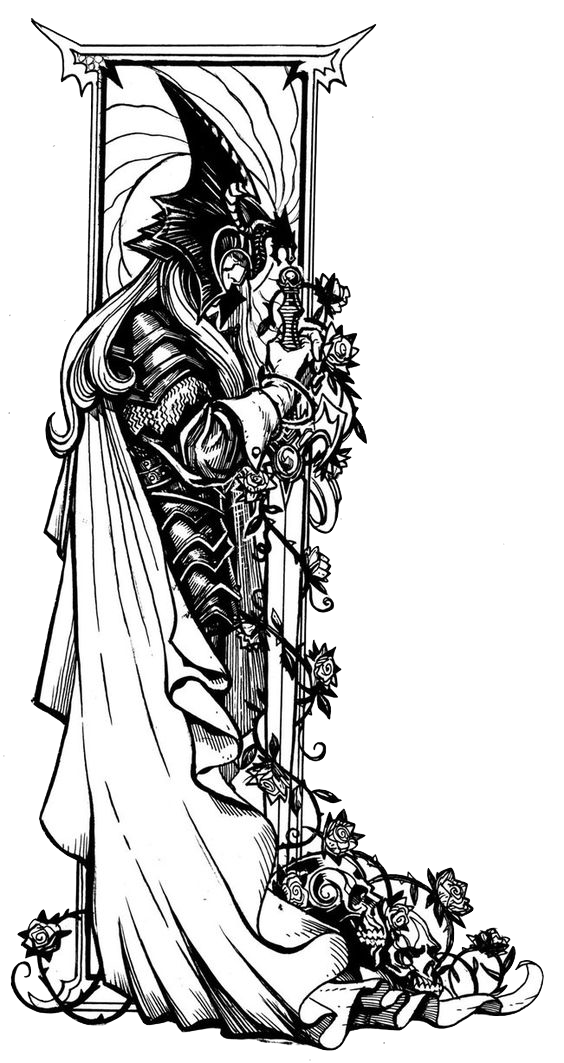
\includegraphics[width=\textwidth]{img/elric.png}
\end{Figure}
    

\end{multicols*}